\begin{flushleft}
\setcounter{page}{1}
\section{Einleitung}
In der folgenden Projektdokumentation stellt der Autor den Projektablauf dar, der im Rahmen seiner
Ausbildung zum Fachinformatiker für Anwendungsentwicklung durchgeführt wurde. Die Durchführung der
Projektarbeit erfolgt bei der Gesellschaft für Systemtechnik, Softwareentwicklung und
Datenverarbeitungsservice mbH \acs{GSSD} in Teltow. Zur Zeit beschäftigt die \acs{GSSD} vier Mitarbeiter und
betreut verschiedene kleine und mittlere Unternehmen als IT-Dienstleister. Des Weiteren ist die \acs{GSSD}
Partner verschiedener Warenwirtschaftssoftware und bietet in diesem Umfeld Anpassung und
Individualisierung an. Zweites Standbein ist der Vertrieb von Hardware für Unternehmen und Privatkunden
sowie deren Installation und Wartung.



\subsection{Projektbeschreibung}
Ein Kunde von der \acs{GSSD} verwendet auf seinen Servern verschiedene Anwendungen, die als
Dienste oder im Hintergrund laufen. Es muss sichergestellt werden, dass diese Anwendungen
ständig funktionieren. Gegenwärtig gibt es ein Überwachungssystem, das nur unvollständige
Zustände anzeigt. Deswegen werde ich ein Überwachungssystem für verschiedene Anwendungen, die auf Servern laufen, entwicklen.
Ziel des Projekts ist es, ein Dashboard zu erstellen, auf dem der Status der Anwendungen angezeigt wird.
Das Überwachungssystem wird als Backend- und Frontend-Anwendung umgesetzt und ermöglicht es dem Administrator, alle verfügbaren Anwendungen sowie deren Zusammenarbeit zu überwachen.
Die Anwendungen selbst liefern regelmäßig Informationen über ihren Zustand und ihre Tätigkeit, die in Datenbanktabellen geschrieben werden.
Das Backend liest diese Informationen aus und bewertet sie, bevor sie im Frontend angezeigt werden.
Der Austausch von Informationen zwischen Frontend und Backend erfolgt über ein Websocket.
Jeder Nutzer kann den Status der Anwendungen auf dem Frontend überprüfen, solange er eine Verbindung hat.
Eine Filterfunktion ermöglicht es dem Backend, die Ausgabe einzuschränken.



\subsection{Projektziel}
Ziel ist die Erstellung einer Überwachung für ein System von Anwendungen. Auf einem Dashboard sollen die Status der Anwendungen in Echtzeit dargestellt werden.
Die Umsetzung wird als Überwachungssystem realisiert, die es dem Administrator ermöglicht, alle verfügbaren Anwendungen auch in ihrer Zusammenarbeit zu überwachen.
Die einzelnen Anwendungen müssen regelmäßig Informationen über ihren Zustand und ihre aktuelle Tätigkeit liefern. Diese Informationen schreiben die Anwendungen in Datenbanktabellen.
Ein Backend liest die Daten aus der Datenbank, bewertet sie und zeigt die Ergebnisse im Frontend. Über ein Websocket werden die benötigten Informationen zwischen Frontend und Backend
ausgetauscht. Auf dem Frontend kann der aktuelle Status von Anwendungen von jedem Nutzer überprüft werden, solange dieser eine Verbindung zum Frontend aufbauen kann.
Über eine Filterfunktion kann die Ausgabe vom Backend eingeschränkt werden. Der User soll in der Lage sein, neue Sensoren zu registrieren. \\ Das Überwachungssystem wird mit den Programmiersprachen HTML, VueJs, CSS, Bash, SQL, NodeJs realisiert.
Die Anwendung wird vom Administrator überwacht und bei bestimmten Fehlermeldungen (Bsp.: Datenbank-Überlastung oder Anwendungsausfall) wird er auf geeignete Weise aufmerksam gemacht.
Somit kann der Administrator reagieren.



\subsection{Projektbegründung}
Die Überwachung von Anwendungen und Systemen ist ein entscheidender Aspekt im Bereich der Informationstechnologie,
da sie eine frühzeitige Erkennung von Fehlern und Problemen ermöglicht, bevor diese sich auf den Betrieb und die Verfügbarkeit der Anwendungen auswirken können.
Ein effektives Überwachungssystem ermöglicht es dem Administrator, die Gesamtleistung des Systems im Blick zu behalten,
den Zustand der einzelnen Komponenten zu überwachen und schnell auf auftretende Probleme zu reagieren.
Dadurch verbessert sich die Qualität und Verfügbarkeit von Anwendungen und die Kundenzufriedenheit steigt.
Durch die Implementierung eines solchen Überwachungssystems können wir sicherstellen,
dass Anwendungen und Systeme stets zuverlässig und fehlerfrei funktionieren.
Wir können schnell auf mögliche Probleme reagieren,
bevor sie sich auf den Betrieb auswirken. Somit tragen wir Gewährleistung der Verfügbarkeit des IT-Systems bei somit haben wir einen reibungslosen IT-Infrastrukturbetrieb, was die Kundenzufriedenheit steigert.

\subsection{Projektschnittstellen}
Das Projekt umfasst die folgenden Schnittstellen:
\begin{itemize}
	\item Geschäftsführung: Der Geschäftsführer der Abteilung, für die das Überwachungssystem implementiert wird, muss über den Fortschritt des Projekts informiert werden und Entscheidungen treffen können, die das Projekt beeinflussen.
	\item IT-Abteilung: Die IT-Abteilung ist für die technische Umsetzung des Projekts verantwortlich und muss eng mit dem Projektteam zusammenarbeiten.
	\item Externe Dienstleister: Falls externe Dienstleister in die IT-Infrastruktur des Unternehmens eingebunden sind, müssen Schnittstellen definiert werden, um sicherzustellen, dass das Überwachungssystem auch auf diesen Systemen funktioniert.
	\item Benutzer: Die Benutzer des Systems müssen über Änderungen informiert und in das Projekt eingebunden werden, um sicherzustellen, dass das Überwachungssystem den Anforderungen der Benutzer entspricht.
	\item Datenbanken und Anwendungen: Das Überwachungssystem muss in der Lage sein, mit anderen Datenbanken und Anwendungen zu kommunizieren, um die erforderlichen Informationen zu sammeln und zu verarbeiten.
	\item Netzwerk- und Sicherheitsinfrastruktur: Die Implementierung des Überwachungssystems erfordert möglicherweise Änderungen an der Netzwerk- und Sicherheitsinfrastruktur des Unternehmens, die von anderen Abteilungen verwaltet werden. Daher müssen Schnittstellen definiert werden, um sicherzustellen, dass alle beteiligten Parteien informiert und beteiligt sind.
\end{itemize}
Die Umsetzung der Schnittstellen erfolgt in enger Zusammenarbeit zwischen dem Projektteam und den beteiligten Parteien. Es müssen klare Verantwortlichkeiten und Kommunikationswege definiert werden, um sicherzustellen, dass alle beteiligten Parteien über den Fortschritt des Projekts informiert sind und dass Probleme schnell gelöst werden können.



\subsection{Projektbegrenzung}
\begin{itemize}
	\item Das Bauen der Sensoren ist kein Bestandteil des Projekts.
	\item Das Projekt konzentriert sich ausschließlich auf die Überwachung von Anwendungen und Systemen innerhalb der internen IT-Infrastruktur des Unternehmens und auf externe Systeme oder Dienstleistungen.
	\item Das Überwachungssystem wird auf alle möglichen Geräte oder Server innerhalb der internen IT-Infrastruktur des Unternehmens und auch auf externe Systeme oder Dienstleistungen implementiert, die von hoher Priorität sind.
	\item Das Projekt beinhaltet keine Anpassungen an bestehende Anwendungen oder Systeme, sondern konzentriert sich ausschließlich auf die Implementierung eines Überwachungssystems.
	\item Das Budget für das Projekt ist begrenzt und schließt keine umfangreichen Änderungen an der IT-Infrastruktur oder den Anwendungen ein.
	\item Die Implementierung des Überwachungssystems wird innerhalb eines bestimmten Zeitrahmens abgeschlossen, um sicherzustellen, dass es so schnell wie möglich in Betrieb genommen werden kann.
	\item Das Projekt umfasst keine Schulungen für Benutzer oder Mitarbeiter, sondern konzentriert sich auf die technischen Aspekte der Implementierung des Überwachungssystems.
	\item Das Überwachungssystem wird nur von einem bestimmten Team oder einer bestimmten Abteilung innerhalb des Unternehmens genutzt und nicht von der gesamten Belegschaft.
\end{itemize}


\subsection{User-Cases}
\begin{itemize}
	\item Das Überwachungssystem soll dem Administrator die Möglichkeit geben, den aktuellen Zustand des Systems mit einem Blick zu beurteilen und frühzeitig auf potenzielle Probleme hinzuweisen.\\
Akteur
\begin{itemize}
	\item Administrator: verantwortlich für die Überwachung des Systems und das Beheben von Problemen.
\end{itemize}
Beschreibung:
\begin{enumerate}
	\item Der Administrator öffnet das Dashboard des Überwachungssystems.
	\item Das Dashboard zeigt eine Übersicht aller verfügbaren Anwendungen und deren aktuellen Zustand an.
	\item Der Administrator kann die Liste der Anwendungen nach verschiedenen Kriterien filtern, um nur relevante Informationen anzuzeigen.
	\item Für jede Anwendung wird eine Bewertung angezeigt, die auf dem aktuellen Zustand und anderen Faktoren basiert.
	\item Wenn eine Anwendung einen kritischen Zustand erreicht oder ein Problem auftritt, wird der Administrator benachrichtigt.
	\item Der Administrator kann auf die Benachrichtigung reagieren, indem er das Problem löst oder einen anderen Schritt unternimmt, um das System wieder in den Normalzustand zu versetzen.
	\item Der Administrator kann das Überwachungssystem anpassen, indem er die Bewertungsfaktoren für die Anwendungen ändert oder neue Anwendungen hinzufügt.
\end{enumerate}
Alternativszenarien:
\begin{itemize}
	\item Wenn das Dashboard nicht korrekt geladen werden kann, wird der Administrator über das Problem informiert und kann versuchen, das Problem zu lösen oder den technischen Support kontaktieren.
	\item Wenn das Überwachungssystem nicht alle erforderlichen Informationen von den Anwendungen empfangen kann, wird der Administrator benachrichtigt und kann das Problem beheben oder die Anwendungen anpassen.
	\item Wenn das Überwachungssystem nicht auf potenzielle Probleme hinweist, die der Administrator erwartet hat, kann der Administrator die Bewertungsfaktoren überprüfen und anpassen, um sicherzustellen, dass alle relevanten Faktoren berücksichtigt werden.
\end{itemize}
\item Die Entwickler können neue Sensoren registrieren.
\end{itemize}


\section{Projektplanung}
\subsection{Projektorganisation}
Geleitet wird das Projekt durch den Autor. Ebenso erfolgt durch ihn die Ausarbeitung des Pflichtenheftes
auf Grundlage des Lastenheftes Anhang A.1: Lastenheft auf Seite II, die daraus folgende Erarbeitung der
einzelnen Komponenten und Prozessketten sowie Aktivitäten im Gesamtprozess.\\
\subsection{Projektphasen}

Zur Durchführung des Projektes standen 80 Stunden zur Verfügung. Für die Ausarbeitung des Konzeptes
wird die meiste Zeit eingeplant. Eine ausführliche Projektplanung ist im voraus nötig, allerdings kann auf
Grund fehlender Erfahrung keine genaue Zeit geschätzt werden, es sind 15 Stunden angesetzt. Da der
Autor zum Zeitpunkt der Durchführung dieser Projektarbeit mit den anzubindenden Komponenten und
Problemen bei der täglichen Arbeit in der \acs{GSSD} vertraut ist, wird ein Zeitaufwand von 6 Stunden für die
Analysephase als realistisch eingeschätzt. Die weiteren Phasen werden als unkritisch eingestuft und
sollten in der Ausarbeitung um maximal eine Stunde je Phase abweichen.\\





Tabelle 1 zeigt die grobe Zeitplanung aus dem Projektantrag.




Dem Anhang A.2: Detaillierte Zeitplanung auf Seite III kann die detaillierte Zeiteinteilung entnommen
werden.

\subsection{Ressourcenplanung}
Für das Projekt werden alle essentiellen Ressourcen durch die Standardausstattung eines IT-Unternehmens abgedeckt. Die Planungsschritte wurden im Büro der \acs{GSSD} durchgeführt und für die Erstellung des Projektplans standen dem Autor ein PC mit \LaTeX  und WhiteStarUML in der freien Version GNU General Public License version 2.0 (GPLv2) zur Verfügung.
Für die Gestaltung der Benutzeroberfläche wurde das Tool Figma gewählt. Mit seinen umfangreichen Funktionen konnte schnell und effektiv ein ansprechendes Design erstellt werden. Besonders produktiv war die Zusammenarbeit mit dem Auftraggeber durch die Möglichkeit des gemeinsamen Arbeitens in Figma.
Für die Umsetzung des Projekts wurden folgende Ressourcen eingeplant:

\begin{itemize}
\item Personal:
\begin{itemize}
\item Der Autor mit 80 Arbeitsstunden
\item Ein Projektbetreuer (Mitarbeiter der \acs{GSSD}) mit 8 Arbeitsstunden
\end{itemize}
\item Hardware:
\begin{itemize}
\item Ein Notebook mit Zugang zum Intranet und Internet
\end{itemize}
\item Software:
\begin{itemize}
\item Visual Studio Code
\item NodeJs
\item VueJs
\item MariaDB Server/Client
\item WhiteStarUML
\item Figma
\item \LaTeX.
\end{itemize}
\end{itemize}

Um Kosten zu sparen, wurde darauf geachtet, keine kostenpflichtige Software einzuplanen.

\subsection{Entwicklungsprozess}
Für die Gestaltung der Benutzeroberfläche wurde ein agiler Prozess gewählt, um kurzfristig auf die Wünsche des Auftraggebers eingehen zu können. Hierfür fanden regelmäßige Rücksprachen statt.
Für die Entwicklung der Server-Komponenten wurde das Wasserfall-Modell gewählt, da der Autor keine späteren Korrekturen in der Architektur erwartet.


\section{Analysephase}
\subsection{Ist-Analyse}
Der Kunde der GSSD nutzt auf seinen Servern verschiedene Anwendungen als Dienste oder im Hintergrund.
Um sicherzustellen, dass diese Anwendungen ständig funktionieren, wurde ein Überwachungssystem implementiert.
Allerdings gibt es derzeit Probleme mit der Funktionalität des Systems, da es nur unvollständige Zustände anzeigt.
Die Ist-Analyse ergab Schwachstellen im aktuellen Überwachungssystem, die verbessert werden müssen, um die Zuverlässigkeit und Funktionalität der überwachten Anwendungen sicherzustellen.
Die Analyseergebnisse bilden die Grundlage für die Planung und Umsetzung von Maßnahmen zur Verbesserung des Überwachungssystems.

\subsection{Workflow}

\begin{figure}[h]
	\centering
	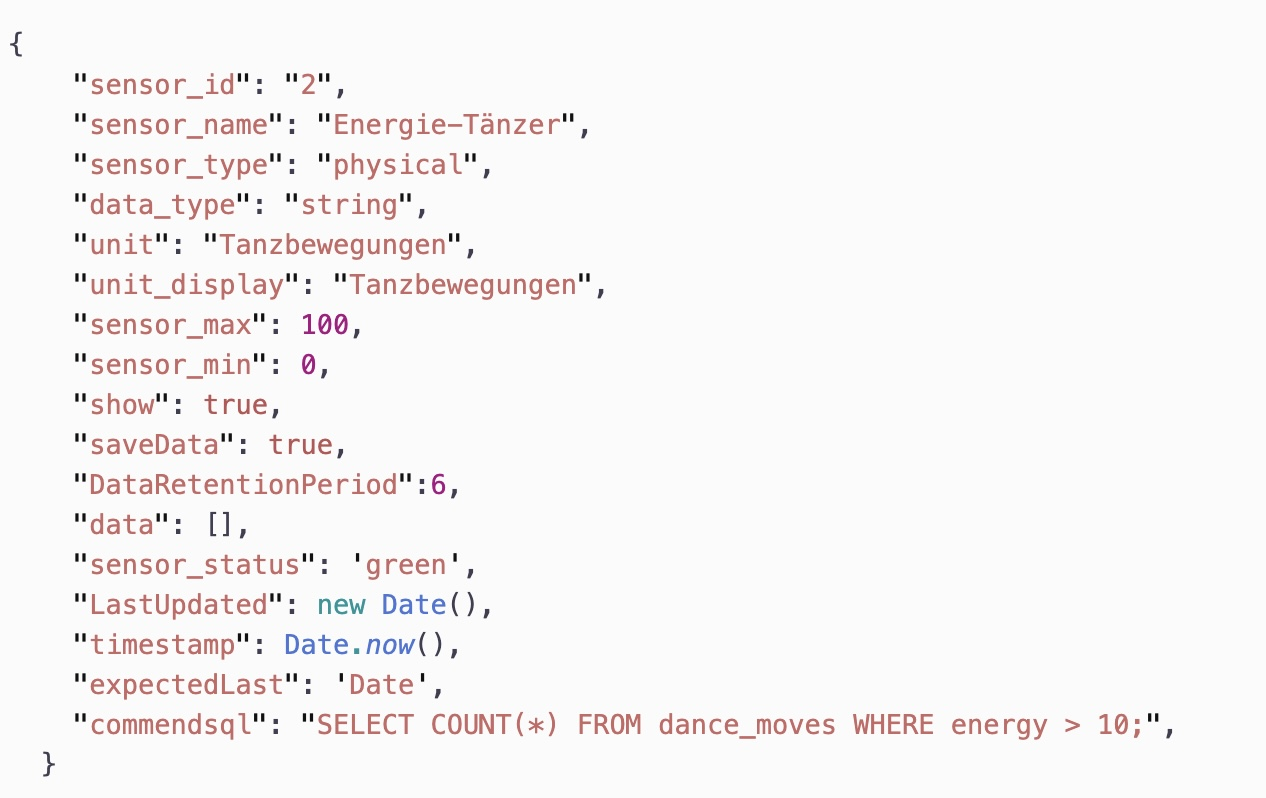
\includegraphics[width=1\textwidth]{img/EnergieTaenzer.png}
	\caption{}
	\label{fig:example}
\end{figure}
Der Code definiert sowohl ein Datenmodell als auch einen Sensor mit verschiedenen Eigenschaften wie Name, Typ, Datentyp, Einheit, Minimum- und Maximumwert, Status, Zeitstempel und weiteren Optionen.\\
Es gibt zwei Arten von Sensoren: echte Sensoren und virtuelle Sensoren. Echte Sensoren senden kontinuierlich Daten an das Backend, während virtuelle Sensoren SQL-Abfragen an das Backend senden, um Daten aus der Datenbank abzurufen.
\\
\begin{enumerate}
	\item Der Prozess der Sensorregistrierung beginnt damit, dass der Sensorbauer eine API-Anfrage an das Backend sendet und seine Anmeldeinformationen übermittelt. Das Backend prüft, ob der Sensor bereits registriert ist. Wenn nicht, wird der Sensor in der Datenbank registriert und die Anmeldeinformationen werden an den Sensorbauer zurückgesendet.
	\item Nach Erhalt der ID des Sensor kann der Sensor regelmäßig Daten an das Backend übermitteln und Konfigurationsdaten abrufen. Das Backend ruft die Konfigurationsdaten des Sensors über die entsprechende ID aus der Datenbank ab und aktualisiert seine Eigenschaften, wie Name, Typ, Datentyp und Einheit.
	\item Der Sensor kann über die show-Eigenschaft angeben, ob er seine Daten an das Frontend senden und über saveData, ob er seine Daten in der Datenbank speichern möchte. Wenn der Sensor Daten senden möchte, aktualisiert er das Datenfeld im Sensor-Modell und sendet es an das Backend.
	\item Das Backend prüft, ob die Daten gemäß der in der variablen DataRetentionPeriodInMonths festgelegten Aufbewahrungsfrist gespeichert werden sollen. Wenn der saveData-Wert auf true gesetzt ist, speichert das Backend die Daten in der Datenbank und aktualisiert den Sensor-Status und den Zeitstempel.
	\item Wenn der Sensor ein virtueller Sensor ist, kann er über die commendsql-Eigenschaft SQL-Abfragen an das Backend senden, um Daten aus der Datenbank abzurufen. Das Backend führt die Abfrage aus und sendet das Ergebnis an den virtuellen Sensor.
	\item Das Frontend empfängt die Daten von den aktiven Sensoren und aktualisiert die Benutzeroberfläche entsprechend. Das Backend überwacht den Status der Sensoren und informiert den Sensorbauer über Probleme, die auftreten könnten, wie z.B. Sensorausfälle oder Datenbankfehler.
	\item Der Sensorbauer kann über die API auch neue Sensoren registrieren, bestehende Sensoren aktualisieren oder löschen sowie weitere Konfigurationen durchführen. Das Backend stellt hierfür entsprechende Funktionen bereit.
\end{enumerate}



\subsection{Soll-Analyse}
Die Soll-Analyse beschreibt die Anforderungen an das Überwachungssystem, die der Kunde an das System stellt.
Die Anforderungen an das Überwachungssystem sind in der Tabelle 2 aufgeführt.\\
Alle relevanten Anwendungen auf den Servern des Kunden
werden überwacht. Durch ein zuverlässige Erkennen von Fehlern oder Ausfällen
wird der Administrator benachrichtigt. Das Überwachungssystem ist einfach konfiguratiert und leicht zu verwalten.
Zusätzlich sollten auch bestimmte Leistungsmerkmale definiert werden, um sicherzustellen, dass das Überwachungssystem den Anforderungen des Kunden entspricht.
Hierzu können beispielsweise die maximale Anzahl der zu überwachenden Anwendungen, die Reaktionszeit bei Fehlermeldungen und die Verfügbarkeit des Überwachungssystems zählen.

\begin{table}[h]
	\centering
	\begin{tabular}{ l l }
	\hline
	\rowcolor{babyblue}
	\textbf{Anforderung} & \textbf{Beschreibung} \\
	\rowcolor{Gray}
	\textbf{Funktional} & \\
	Diensteüberwachung & Überwachung der Dienste, die auf den Servern laufen \\
	Alarmierung & Benachrichtigung im Falle von Störungen \\
	Protokollierung & Aufzeichnung von Zustandsänderungen und Störungen \\
	Registrieren & neue Sensor registrieren \\
	\rowcolor{Gray}
	\textbf{Nicht-Funktional} & \\
	Benutzerfreundlichkeit & Einfache Bedienbarkeit des Systems \\
	Zuverlässigkeit & Hohe Verfügbarkeit und Genauigkeit des Überwachungssystems \\
	\rowcolor{Gray}
	\textbf{Qualität} & \\
	Skalierbarkeit & Möglichkeit zur Erweiterung des Systems \\
	Flexibilität & Anpassung an unterschiedliche Anforderungen des Kunden \\
	\rowcolor{Gray}
	\textbf{Leistung} & \\
	Echtzeitüberwachung & Echtzeitüberwachung der Zustände \\
	Ressourcenschonung & Geringer Ressourcenverbrauch auf den überwachten Servern \\  \hline
	\end{tabular}
	\caption{Anforderungen an das Überwachungssystem}
\end{table}

\subsection{Wirtschaftlichkeitsanalyse}
\subsubsection{Checkmk}
Checkmk ist eine Monitoring-Lösung für IT-Infrastrukturen, die es Unternehmen ermöglicht, ihre IT-Systeme zu überwachen und Probleme frühzeitig zu erkennen.
Das System nutzt eine Vielzahl von Sensoren, um Informationen über die Systeme zu sammeln und an die Checkmk-Server zu übermitteln.
Checkmk unterstützt auch eine REST-API, die es ermöglicht, auf die Informationen von Checkmk zuzugreifen und diese in anderen Anwendungen zu nutzen.
\\
Die Checkmk-API ermöglicht es, Daten von Checkmk zu extrahieren, um sie in anderen Anwendungen zu nutzen.
Dies kann zum Beispiel dazu genutzt werden, um Informationen über Systemauslastung oder Status von Diensten zu sammeln und in einer anderen Anwendung anzuzeigen.
Die API kann auch dazu genutzt werden, um automatisierte Aktionen auszuführen, wie zum Beispiel das Neustarten von Diensten, wenn diese ausfallen.


\subsubsection{Weitere Fremdsoftware}
Das Projekt ist eine aufregende Expedition in die Welt der Software-Entwicklung.
Es ist eine Herausforderung voller Chancen und Möglichkeiten, bei der das Ziel darin besteht,
eine maßgeschneiderte Lösung zu kreieren, die perfekt auf die Bedürfnisse des Kunden zugeschnitten ist.
Ich werde dabei innovative Technologien und kreative Ansätze einsetzen, um die besten Ergebnisse zu erzielen.
Die Reise ist wie eine Expedition ins Unbekannte, bei der das Ziel zwar klar ist, der Weg dorthin jedoch voller Überraschungen steckt.
Doch mit jeder Herausforderung werde ich wachsen und wertvolle Erfahrungen sammeln, um schlussendlich ein Projekt zu liefern, das den Kunden in Begeisterung versetzt.


\subsubsection{Eigenentwicklung}
Die Eigenentwicklung von Software bietet zahlreiche Vorteile. Einer davon besteht darin, dass die Software speziell auf die Anforderungen und Bedürfnisse des Anwenders zugeschnitten werden kann. Dadurch kann eine optimale Lösung für das zugrunde liegende Problem gefunden werden. Zudem kann der Workflow bei der Benutzung der Software im Voraus geplant und anschließend umgesetzt werden.
\\
Ein weiterer Vorteil besteht darin, dass bei der Eigenentwicklung der Software die volle Kontrolle über den Code und dessen Implementierung besteht. Dies ermöglicht es, Fehlerquellen schnell zu identifizieren und zu beheben. Auch können neue Funktionalitäten und Erweiterungen leichter implementiert werden, da der Code von Grund auf bekannt ist.
\\
Zudem bietet die Eigenentwicklung von Software die Möglichkeit, die Software kontinuierlich zu verbessern und anzupassen, um den sich ändernden Anforderungen und Bedürfnissen des Anwenders gerecht zu werden.

\subsubsection{Projektkosten}
Im Rahmen dieses Projekts sind insgesamt 80 Stunden für die Umsetzung des Konzepts veranschlagt. Basierend auf einem Stundensatz von 10 € für einen erfahrenen Programmierer und zusätzlichen Gemeinkosten in Höhe von 35 €, belaufen sich die Gesamtkosten auf \textbf{1080,00 €}.
\begin{center}
	\begin{tabular}{ l r r r }
	\rowcolor{babyblue}
	\textbf{Vorgang} & \textbf{Zeit} & \textbf{Kosten pro Stunde} & \textbf{Kosten} \\
	Auszubildender & 80 h & 10,00 € & 800,00 €  \\
	\rowcolor{Gray}
	Mitarbeiter & 8 h & 35,00 € & 200,00 €  \\ \hline
	\rowcolor{babyblue}
	 & & & \textbf{1080,00 €}  \\
	\end{tabular}
	\captionof{table}{Kostenaufstellung}
\end{center}
In diesem Projekt wird die Open-Source-Software NodeJs und VueJs genutzt, die kostenfrei verfügbar sind. Allerdings sind zusätzliche Kosten unvermeidbar, da sie direkt mit der Implementierung des Konzepts und der Nutzung von NodeJs und VueJs zusammenhängen. Zu diesen Kosten gehören die Erstellung des Backends zur Nutzung von NodeJs und die Erstellung des Frontends zur Nutzung von VueJs. Darüber hinaus muss ein eigenes Überwachungssystem entwickelt werden, da keine Alternativen von Checkmk oder anderen Fremdsoftware den speziellen Anforderungen entsprechen, die im Anhang A.1: Lastenheft auf Seite II festgelegt sind.\\
\textbf{Kostenschätzung der Projektumsetzung} Wird die Implementierung der nachfolgenden Komponenten
von einem Programmierer der GSSD durchgeführt, wird ebenfalls mit dem oben genannten Stundensatz
von 10 €, zzgl. 35 € Gemeinkosten kalkuliert.\\
Für die Entwicklung der Backend werden 3 Stunden veranschlagt (135 €).Es werden mit 8 h für die
Entwicklung des Backend gerechnet (360 €). Das bereitgestellte Backend, muss bei
bestehender Eigensoftware implementiert werden, sofern die Überwachungssystems benutzt werden soll. Dafür wird ein
Aufwand von ca. einem Arbeitstag pro Programm geschätzt (je 408 €).\\
Die für die Fremdsoftware zusätzlich benötigte Checkmk, muss für jede Fremdsoftware speziell
angepasst werden. Pro Fremdsoftware wird mit einem Aufwand von mindestens zwei Arbeitstagen
gerechnet (je 816 €).\\
Die im Rahmen der Projektarbeit erwähnte grafische Benutzeroberfläche, muss von Grund auf entwickelt
werden. Für die Erstellung von ca. 80 der Funktionalität und damit dem erreichen des ersten Milestone,
werden inklusive Tests ca. 10 Arbeitstage berechnet (4080 €). Sofern die bis dahin realisierte
Funktionalität nicht als ausreichend bewertet wird, können in weiteren Schritten fehlende Funktionen
ergänzt werden. Aufwandsschätzungen müssen daraufhin erneut stattfinden.
Für die abschließende Schulung sind einmalig 4 Stunden geplant (204 €).\\
Da das Projekt und auch alle davon abhängigen Prozesse keinem Kundenprojekt direkt zugeordnet
werden können, müssen die Projektkosten mit zukünftigen Projekten verrechnet werden, sie fallen daher
zunächst als variable Kosten im Unternehmen an.

\subsubsection{Amortisationsdauer}
Die Nutzung des Eigenentwicklungs-Überwachungssystems erfordert keine weiteren Lizenzgebühren.
Allerdings ist die Implementierung des Systems nicht Teil des Projekts und die damit verbundenen Kosten sind nicht enthalten.
Das Überwachungssystem kann jedoch dazu beitragen, dass Sensoren fast vollautomatisch gebaut werden können, was zu erheblichen Zeitersparnissen führt.
Eine Benutzeroberfläche wird in Zukunft auch Kunden die Möglichkeit geben, die komplexen Anwendungen des Systems zu überwachen und dadurch weitere Einsparungen bei Zeit und Kosten zu erzielen.
\subsection{Lastenheft}
Für die Überwachung eines komplexen Systems gibt es verschiedene Ansätze. Ein möglicher Ansatz ist die Erstellung einer Gesamtbewertungsanzeige, die den Zustand des gesamten Systems anzeigt. Dazu können folgende Schritte durchgeführt werden:

\begin{enumerate}
\item Identifikation der relevanten Komponenten und Sensoren
\item Definition von Schwellwerten für jeden Sensor
\item Zusammenfassung der Sensorwerte in einer geeigneten Form
\item Definition von Alarmstufen für jeden Schwellwert
\item Integration von Bewertungsregeln
\item Anzeige der Bewertung auf eine einfache und intuitive Weise
\item Automatische Alarmierung bei kritischen Zuständen des Systems
\item Langzeitanalyse der Sensorwerte für Trends und Muster im Systemverhalten
\item Interaktive Dashboards für detaillierte Ansichten und individuelle Einstellungen.
\end{enumerate}

Durch die Erstellung einer Gesamtbewertungsanzeige können komplexe Systeme effektiv überwacht werden. Die Anzeige sollte auf eine einfache und intuitive Weise dargestellt werden und automatische Alarmierungen bei kritischen Zuständen des Systems ermöglichen. Langzeitanalysen der Sensorwerte können Trends und Muster im Systemverhalten aufdecken und interaktive Dashboards bieten detaillierte Ansichten und individuelle Einstellungsmöglichkeiten.
\section{Entwurfsphase}
\subsection{Zielplattform}
In der Entwurfsphase wurden technische Anforderungen berücksichtigt und eine Architektur erstellt. Das System besteht aus Backend und Frontend, welche über Websockets Daten austauschen. Die Datenbank wurde mit PostgreSQL realisiert und enthält Tabellen für Anwendungsdaten. Das Backend (Node.js, Express) liest und bewertet die Daten und das Frontend (Vue.js, Bootstrap) zeigt sie auf einem Dashboard an. Das System kann Anwendungen hinzufügen und die Filterfunktion einschränken. Die Entwurfsphase hat klare Vorgaben auf Basis der Kundenanforderungen geschaffen, um sicherzustellen, dass das System alle notwendigen Anforderungen erfüllt.
\subsection{Architekturdesign}
\textcolor{red}{\textbf{TODO}}\\
\subsection{Datenbank}
\textcolor{red}{\textbf{Entscheidung Prozess :}}\\
Entscheidung Prozess :
\begin{itemize}
\item \textcolor{red}{\textbf{mysql -> Microsoft-server -> administrationaufwand.}}
\item \textcolor{red}{\textbf{ sql-lite -> mehr aufwand in der programmierung.}}
\item \textcolor{red}{\textbf{ nonsql datenbank -> einfach programmieren, kein Administrationsaufwand}}
\item \textcolor{red}{\textbf{ Mengenbetrachtung -> 100 Aufträge pro jahr sind nicht viel, dann ist das nicht nötwendig einen Datenbank mit server zu bauen.}}
\end{itemize}
\textcolor{red}{\textbf{Der Go-Code für den Datenbankmodel ist im Anhang zu sehen.}}
\subsection{REST-API}
\textcolor{red}{\textbf{TODO}}\\
\subsection{Entwurf der Benutzeroberfläche}
\textcolor{red}{\textbf{Während der Gestaltung der Benutzeroberfläche wurden zunächst einige Mockups erstellt (siehe Anhang für das Web-Frontend-Mockup). Dabei wurde darauf geachtet, dass die Bedienoberfläche bedienbar ist und ansprechend aussieht.}}\\
\subsection{Maßnahmen zur Qualitätssicherung}
\textcolor{red}{\textbf{TODO}}\\
Es wurde Unit- und Widget-Tests zu schreiben, mithilfe derer die Korrektheit  der Implementierung überprüft werden kann.\\
Außerdem wurden regelmäßige Rücksprachen mit dem Leiter der Entwicklungsabteilung geplant, um frühzeitig ungewollte Abweichungen vom Ziel zu vermeiden.\\
Sämtlicher Quellcode der Software wurde unter die GIT-Versionsverwaltung gestellt, um zu jedem späteren Zeitpunkt die Historie der Softwareentwicklung nachvollziehen zu können.
Es wurde eine Continuous Integration (CI) mithilfe von Jenkins realisiert, die nach jedem Push in das GIT-Repository automatisch die Software baut und die Unit- und Widget-Tests ausführt.\\
\subsection{Deployment}
\textcolor{red}{\textbf{TODO}}\\
\subsection{Pflichtenheft}
\textcolor{red}{\textbf{TODO}}\\
Auf der Basis von Lastenheft und im Hinblick auf die vorhandenen Ressourcen wurde einen Pflichtenheft erstellt. Dieses enthielt die präzisierten Anforderungen des Lastenheftes und deren geplanten Umsetzung, sieh im Anhang Abbildung .\\
\section{Implementierungsphase}
\subsection{Vorbereitung des Projektes}
\textcolor{red}{\textbf{TODO}}\\
\subsection{Implementierung des Backendes}
\textcolor{red}{\textbf{TODO}}\\
\subsection{Implementierung des Frontends}
\textcolor{red}{\textbf{TODO}}\\
\subsection{Testen der Anwendung}
\textcolor{red}{\textbf{TODO}}\\
\section{Abnahmephase}
\subsection{Code-Review}
\textcolor{red}{\textbf{Ein Code-Review wurde zuletzt durchgeführt, hier geht es darum, ob die Name der Funktionen und Variablen richtig und sinnvoll geschrieben sind, ob alle tests geschrieben, die notwendig sind, ob die oberfl\"ache sch\"on aussieht und einfach zu bedienen ist und schließlich ob die Funktionalität wie erwünscht funktioniert.}}\\
\subsection{Abnahme}
\textcolor{red}{\textbf{Die Abnahme war kurz, weil eine Rücksprache mit dem Entwicklungsleiter (der Auftragsgeber) immer stattfand .}}\\
\section{Dokumentation}
\textcolor{red}{\textbf{latex parallel}}\\
\section{Fazit}
\subsection{Soll-\/Ist-Vergleich}
\textcolor{red}{\textbf{Durchs Vergleich zwischen dem Produkt was am Ende kommt und dem Lasten Heft, kann man sagen, dass der Produkt alle erwünschten Kriterien erf\"ullt.}}
\\
\end{flushleft}
